\documentclass{uebblatt}

\begin{document}

\maketitle{5}{\emph{Lokal präsentierbare Kategorien: \\ große Kategorien, die
von kleinen Daten erzeugt werden.}}

\begin{aufgabe}{Kompakte Objekte in Modulkategorien}
\begin{enumerate}
\item Zeige, dass ein~$A$-Modul~$M$ genau dann endlich erzeugt ist, wenn der
Funktor~$\Hom(M,\smallplaceholder) : \mathrm{Mod}(A) \to \Set$ mit filtrierten
Kolimiten von Monomorphismen vertauscht, wenn also für jedes filtrierte
Diagramm~$(V_i)_i$, in der die Übergangsabbildungen $V_i \to V_j$ alle injektiv
sind, folgende kanonische Abbildung bijektiv ist.
\[ \colim_i \Hom(M,V_i) \longrightarrow \Hom(M, \colim_i V_i) \]
\vspace{-1.7em}
\item Zeige, dass ein~$A$-Modul~$M$ genau dann endlich präsentiert ist, wenn
der Funktor~$\Hom(M,\smallplaceholder)$ mit beliebigen filtrierten Kolimiten
vertauscht, wenn~$M$ also~$\aleph_0$-kompakt ist.
\end{enumerate}
\end{aufgabe}

\begin{aufgabe}{Kompakte Objekte in der Kategorie der topologischen Räume}
Sei~$X$ ein topologischer Raum, der eine Teilmenge~$A \subseteq X$ besitzt, die
nicht offen ist. Zeige, dass~$X$ in der Kategorie der topologischen Räume
nicht~$\aleph_0$-kompakt ist.
\end{aufgabe}

\begin{aufgabe}{Vertauschbarkeit von filtrierten Kolimiten mit endlichen Limiten}
Sei~$F : \C \times \D \to \Set$ ein Funktor.
\begin{enumerate}
\item Konstruiere einen kanonischen Morphismus~$\psi : \colim\limits_{c \in \C}
\lim\limits_{d \in \D} F(c,d) \to \lim\limits_{d \in \D} \colim\limits_{c \in \C} F(c,d)$.
\item Sei~$\C$ sogar eine filtrierte Kategorie und~$\D$ eine endliche. Zeige, dass dann~$\psi$ ein Isomorphismus ist.
\end{enumerate}
Folgere: Endliche Kolimiten von~$\aleph_0$-kompakten Objekten
sind~$\aleph_0$-kompakt.
\end{aufgabe}

\begin{aufgabe}{Das Theorem von Whitehead für Modellkategorien}
Zeige, dass ein Morphismus zwischen bifasernden Objekten in einer
Modellkategorie genau dann eine Homotopieäquivalenz ist, wenn er eine schwache
Äquivalenz ist.
\end{aufgabe}

\begin{aufgabe}{Morphismen zwischen kofasernden und fasernden Objekten}
\begin{enumerate}
\item
Seien~$X$ ein kofaserndes und~$Y$ ein faserndes Objekt in einer
Modellkategorie~$\M$. Zeige, dass der kanonische Morphismus~$\pi(X,Y) \to
\pi(RX,QY)$ bijektiv ist.
\item Beweise, dass in~$\Ho(\M)$ jeder Morphismus Komposition von Morphismen der
Form~$\gamma(f)$ mit~$f \in \Mor\M$ und Morphismen der Form~$\gamma(f)^{-1}$
mit~$f \in \W$ ist.
\end{enumerate}
\end{aufgabe}

\centering
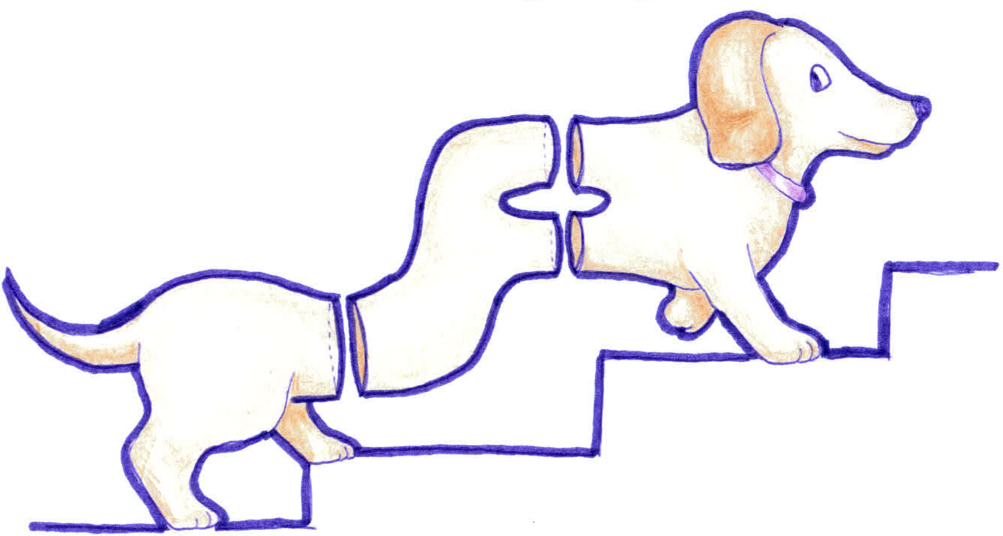
\includegraphics[scale=0.50]{images/tqft}
\par

\end{document}

\begin{aufgabe}{Hom als Delta-Distribution}
Sei~$F : \C^\op \to \Set$ eine Prägarbe und~$c \in \C$. Zeige:
$\Hom_\C(\smallplaceholder, c) \otimes F = F(c)$.
\end{aufgabe}

Zeige, dass die transfinite Komposition von relativen~$\I$-Zellkomplexen
ein relativer~$\I$-Zellkomplex ist.
